\documentclass[a4paper,12pt]{article}
\usepackage[a4paper,top=1.3cm,bottom=2cm,left=1.5cm,right=1.5cm,marginparwidth=0.75cm]{geometry}
%%% Работа с русским языком
\usepackage{cmap}					% поиск в PDF
\usepackage{mathtext} 				% русские буквы в фомулах
\usepackage[T1, T2A]{fontenc}			% кодировка
\usepackage[utf8]{inputenc}			% кодировка исходного текста
\usepackage[english,russian]{babel}	% локализация и переносы

\usepackage{indentfirst} % отступ первой строки после заголовка

\usepackage{graphicx}
\graphicspath{{pictures/}} % путь к папке с фотографиями

\usepackage{wrapfig}
\usepackage{tabularx}

\usepackage{hyperref}
\usepackage[rgb]{xcolor}
\hypersetup{
colorlinks=true,urlcolor=blue
}

%%% Дополнительная работа с математикой
\usepackage{amsmath,amsfonts,amssymb,amsthm,mathtools}
\usepackage{icomma} % "Умная" запятая: $0,2$ --- число, $0, 2$ --- перечисление

%% Номера формул
\mathtoolsset{showonlyrefs,showmanualtags} % Показывать номера только у тех формул, на которые есть \eqref{} в тексте.

%% Шрифты
\usepackage{euscript}	 % Шрифт Евклид
\usepackage{mathrsfs} % Красивый матшрифт

%% Свои команды
\DeclareMathOperator{\sgn}{\mathop{sgn}}

%% Перенос знаков в формулах (по Львовскому)
\newcommand*{\hm}[1]{#1\nobreak\discretionary{}
{\hbox{$\mathsurround=0pt #1$}}{}}

%%% Заголовок
\author{Волков Никита Алексеевич}
\title{Лабораторная работа №1.4.1-B

Изучение экспериментальных погрешностей на примере физического маятника
}
\date{\today}

\begin{document}

\begin{titlepage}
	\begin{center}
		{\large МОСКОВСКИЙ ФИЗИКО-ТЕХНИЧЕСКИЙ ИНСТИТУТ (НАЦИОНАЛЬНЫЙ ИССЛЕДОВАТЕЛЬСКИЙ УНИВЕРСИТЕТ)}
	\end{center}
	\begin{center}
		{\large Физтех-школа аэрокосмических технологий}
	\end{center}
	
	
	\vspace{4.5cm}
	{\huge
		\begin{center}
			{\bf Отчёт о выполнении лабораторной работы 1.4.1-B}\\
			Изучение экспериментальных погрешностей\\
			на примере физического маятника
		\end{center}
	}
	\vspace{2cm}
	\begin{flushright}
		{\LARGE Автор:\\ Волков Никита Алексеевич \\
			\vspace{0.2cm}
			Б03-103}
	\end{flushright}
	\vspace{8cm}
	\begin{center}
		Долгопрудный 2021
	\end{center}
\end{titlepage}

\tableofcontents

\newpage


\section{Введение}


\textbf{Цель работы:} 1) на примере измерения периода свободных колебаний физического маятника познакомиться с систематическими и случайными погрешностями, прямыми и косвенными измерениями; 2) проверить справедливость формулы для периода колебаний физического маятника и определить значение ускорения свободного падения; 3) убедиться в справедливости теоремы Гюйгенса об обратимости точек опоры и центра качания маятника; 4) оценить погрешность прямых и косвенных измерений и конечного результата.
\medskip

\textbf{В работе используются:} металлический стержень с опорной призмой; дополнительный груз; закреплённая на стене консоль; подставка с острой гранью для определения цента масс маятника; секундомер; счётчик колебаний (механический или
электронный); линейки металлические различной длины; штангенциркуль; электронные весы; математический маятник (небольшой груз, подвешенный на нитях).
\medskip


\section{Теоретические сведения}

\begin{wrapfigure}{r}{0.25\textwidth}
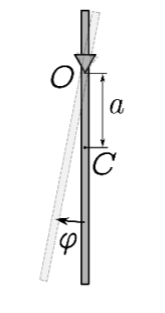
\includegraphics[width=0.25\textwidth]{fiz.maytnik.png}
\caption{Стержень как физический маятник} \label{fiz.maytnik}
\end{wrapfigure}


Физическим маятником называют твёрдое тело, способное совершать колебания в вертикальной плоскости,
будучи подвешено за одну из своих точек в поле тяжести.
Основное отличие физического маятника от математического в том, что маятник не является точечным объектом,
а представляет собой совокупность жёстко связанных точечных масс. В данной работе в качестве такого маятника
используется тонкий однородный металлический стержень, подвешиваемый в некоторой точке с помощью небольшой опорной призмы (см. рис. \eqref{fiz.maytnik}). Острое ребро
призмы, опирающееся на подставку, задаёт ось качания
(или вращения) маятника.


Закон, описывающий вращательное движение твёрдого тела вокруг фиксированной оси, аналогичен второму закону Ньютона.

\begin{equation}\label{moment_sili_1}
M = \dfrac{dL}{dt},
\end{equation}

где $M$ - момент силы, $L = mr^{2}\omega$ - момент импульса. Величину $J = mr^{2}$ называют моментом инерции точечного тела. При постоянном $J$ уравнение \eqref{moment_sili_1} можно записать как

\begin{equation}\label{moment_sili_2}
M = J\dfrac{d\varphi}{dt}
\end{equation}


В случае твёрдого тела, состоящего из совокупности материальных точек, вращающихся вокруг фиксированной оси,
уравнение \eqref{moment_sili_2} сохраняет свой вид, но под моментом инерции следует понимать сумму (или интеграл) по всем точкам тела:

\begin{equation}\label{moment_inercii}
J = \sum_i m_ir_i^2,
\end{equation}
где $r_i$ — расстояние от точки массой $m_i$ до оси вращения.  Момент
инерции тонкого стержня массой $m$ и длиной $l$, вращающегося вокруг оси,
проходящей через центр масс, равен

\begin{equation}\label{moment_inercii_sterjnya}
J_C = \dfrac{ml^2}{12}
\end{equation}

А момент инерции стержня, подвешенного на расстоянии $a$ от центра масс,
может быть вычислен по теореме Гюйгенса–Штейнера:

\begin{equation}\label{moment_inercii_sterjnya}
J_C = \dfrac{ml^2}{12} + ma^2
\end{equation}


Момент силы тяжести, действующей на стержень, при небольших углах отклонения $\varphi \ll 1$ равен

\begin{equation}\label{moment_sili_mayatnika}
M = -mga \sin \varphi \approx -mga \varphi.
\end{equation}


Возвращающий момент сил, пропорциональный величине его отклонения от равновесия, поэтому при малых амплитудах отклонения движение свободного физического маятника будет иметь характер гармонических колебаний, аналогично колебаниям груза на пружине или математического маятника. Период колебаний произвольного физического маятника:

\begin{equation}\label{period_kolebaniy_proizvolnogo_mayatnika}
T = 2\pi\sqrt{\dfrac{J}{mga}}.
\end{equation}


\begin{wrapfigure}{r}{0.15\textwidth}
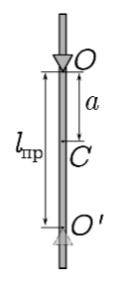
\includegraphics[width=0.15\textwidth]{prived_dlina.png}
\caption{К теореме Гюйгенса} \label{prived_dlina_photo}
\end{wrapfigure}


Для стержня длиной $l$, подвешенного на расстоянии $a$ от центра, c учётом \eqref{moment_inercii_sterjnya} получаем:

\begin{equation}\label{period_kolebaniy_mayatnika}
T = 2\pi\sqrt{\dfrac{ \dfrac{l^2}{12} + a^2 }{ga}}.
\end{equation}


Определим так называемую приведённую длину физического маятника:

\begin{equation}\label{prived_dlina}
l_{\text{пр}} = a + \dfrac{l^2}{12a}.
\end{equation}

Смысл этой длины в том, что физический маятник длиной $l$, подвешенный в точке $a$, имеет тот же период малых колебаний, что и математическиймаятник длиной $l_{\text{пр}}$.


С понятием «приведённой длины» связана следующая теорема (Гюйгенса). Рассмотрим точку $O'$, отстоящую от точки опоры $O$ на расстояние $l_{\text{пр}}$ вдоль стержня (эту точку иногда называют центром качания физического маятника). Если маятник подвесить за точку $O'$, то период его качания не изменится. Иными словами, точка опоры и центр качания маятника взаимно обратимы.


\begin{wrapfigure}{r}{0.4\textwidth}
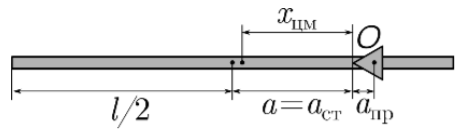
\includegraphics[width=0.4\textwidth]{smeschenie_CM.png}
\caption{Смещение центра масс из-за подвесной призмы} \label{smeschenie_CM}
\end{wrapfigure}


Также можно учесть влияние подвесной призмы. Формула \eqref{period_kolebaniy_mayatnika} получена в предположении, что подвес маятника является материальной точкой. На самом же деле маятник подвешивается с помощью треугольной призмы конечного размера, поэтому использование \eqref{period_kolebaniy_mayatnika} может привести к систематической погрешности результата.Поскольку расстояние $a_{\text{пр}}$ трудно поддаётся непосредственному измерению, можно исключить его, измеряя положение центра масс всей системы. Пусть $x_{\text{ц}}$ — расстояние от центра масс системы до точки подвеса. По определению имеем

\[ x_{\text{ц}} = \dfrac{ m_{\text{ст}}a_{\text{ст}} - m_{\text{пр}}a_{\text{пр}} }{ m_{\text{ст}}m_{\text{пр}} } \]

(«минус» учитывает положение призмы). Исключая отсюда $a_{\text{пр}}$, получим
формулу для периода с нужной нам поправкой:

\begin{equation}\label{period_kolebaniy_mayatnika_14}
T = 2\pi \sqrt{ \dfrac{ \dfrac{l^2}{12} + a^2 }{ g (1 + \dfrac{m_{\text{пр}}}{m_{\text{ст}}}) x_{\text{ц}} } }.
\end{equation}


Таким образом, для более точного измерения g следует для каждого положения призмы измерять не только величину $a$ — положение призмы относительно центра масс стержня), но и расстояние $x_{\text{ц}}$ — положение центра масс стержня с призмой относительно призмы (см рис. \ref{smeschenie_CM})


\section{Оборудование и эксперементальные погрешности}

\noindent \textbf{Секундомер:} $\delta_\text{с} = \pm 0,01$ с \\
\textbf{Весы:} $\delta_\text{в} = \pm 0,5$ г \\
\textbf{Линейка:} $\delta_\text{лин} = \pm 0,5$ мм \\
\textbf{Штангенциркуль:} $\delta_\text{шт} = \pm 0,05$ мм \\

\newpage


\section{Результаты измерений и обработка данных}

\subsection{Предварительные измерения и рассчеты}

\begin{wrapfigure}{r}{0.15\textwidth}
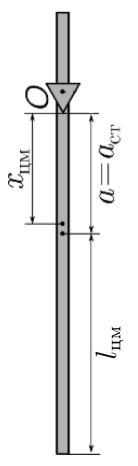
\includegraphics[width=0.15\textwidth]{izmereniya_1.png}
\caption{Измеряемые длины} \label{izmereniya_1}
\end{wrapfigure}

\begin{table}[]
\caption{\textit{Первоначальные измерения}}
\label{nach_izm}
\begin{center}
	\begin{tabular}{|l|l|l|l|}
	\hline
                       & \textit{Измерение} & $\sigma$   & $\varepsilon$, \textit{\%} \\ \hline
	$l$, мм  & 1000      & 0,5 & 0,05  \\ \hline
	$l_{\text{цм}}$, мм & 500       & 0,5 & 0,10  \\ \hline
	$a$, мм                  & 250       & 0,5 & 0,20  \\ \hline
	$x_{\text{ц}}$, мм                 & 231       & 0,5 & 0,22  \\ \hline
	$m_{\text{ст}}$, г & 1022,4    & 0,1 & 0,01  \\ \hline
	$m{\text{пр}}$, г  & 74,0      & 0,1 & 0,14  \\ \hline
	\end{tabular}
\end{center}
\end{table}

Сначала необходимо измерить характеристики установки: длину стержня $l$, расстояние до центра масс пустого стержня $l_{\text{цм}}$, положение $a$ острия призмы относительно центра масс стержня, положение центра масс конструкции $x_{\text{ц}}$, массу пустого стержня $m_{\text{ст}}$ и массу призмы $m{\text{пр}}$. Для каждой величины рассчитаем относительную погрешность. Результаты измерений представленны в таблицы \eqref{nach_izm}. По данным таблицы период колебаний маятника имеет смысл измерять с относительной погрешностью $\varepsilon_{max} = 0.22 \%$.


Необходимо провести предварительный опыт по измерению периода колебаний, чтобы уббедится, что маятник качается без помех, призма не проскальзывает, и колебания затухают слабо. Время $n = 10$ полных колебаний маятника $t = 15,32 c$. Вычислим период колебаний $T = t/n = 15,32/10 \approx 1,53 с$ и по формуле \eqref{period_kolebaniy_mayatnika_14} рассчитаем предварительное значение $g \approx 9.9 м/с^2$.  Оно мало отличается от табличного значения.


\subsection{Определение погрешности измерения времени}

Для экспериментального определения случайной погрешности измерения времени с помощью секундомера было проведено 10 измерений времени $n = 10$ колебаний. Результаты измерений представленны в таблице \ref{izm_vremeni}.


\begin{table}[h]
\caption{\textit{Измерение времени}}
\label{izm_vremeni}
\begin{tabular}{|l|l|l|l|l|l|l|l|l|l|l|}
\hline
N опыта & 1     & 2  & 3     & 4     & 5     & 6     & 7     & 8     & 9     & 10    \\ \hline
t, с    & 15,34 & 15 & 15,41 & 15,52 & 15,08 & 15,33 & 15,23 & 15,34 & 15,45 & 15,34 \\ \hline
\end{tabular}
\end{table}

В таблице \ref{pogr_izm_vremeni} представленны среднее значение полученных результатов $t_{\text{ср}}$, случайная погрешность измерения времени $\sigma_{\text{случ}}$, вычисляемая по формуле:

\begin{equation}\label{sigma_sluch}
\sigma_{\text{случ}} = \sqrt{  \dfrac{1}{N-1} \sum_i(t_i - t_{\text{ср}}) },
\end{equation}

а также систематическая погрешность секундомера $\sigma_{\text{сист}}$ и полная погрешность измерения времени $\sigma_{\text{полн}}$. Т.к. $\sigma_{\text{случ}}  \gg \sigma_{\text{сист}}$, то $\sigma_{\text{полн}} \approx \sigma_{\text{случ}}$.

\begin{table}[]
\caption{\textit{Погрешность измерения времени}}
\label{pogr_izm_vremeni}
\begin{center}
\begin{tabular}{|l|l|l|l|}
\hline
$t_{\text{ср}}$   & $\sigma_{\text{случ}}$  & $\sigma_{\text{сист}}$  & $\sigma_{\text{полн}}$  \\ \hline
15,30 & 0,16 & 0,01 & 0,16 \\ \hline
\end{tabular}
\end{center}
\end{table}


Чтобы относительная погрешность измерения периода соответствовала $\varepsilon_{max} = 0.22 \%$ при $\sigma_{\text{t}} = 0.16 c$, необходимо, чтобы количество измерений было

\[ n = \dfrac{\sigma_{\text{t}}}{\varepsilon_{T} T} = \{\varepsilon_{T} = \varepsilon_{max}\} = \dfrac{0.16}{0.0022 \cdot 1.53} \approx 48 \].

Таким образом, для достижения требуемой точности достаточно выполнить однократное измерение времени $n \approx 48$ колебаний.



\subsection{Опыт по определению ускорения свободного падения}

Проведем измерение периода колебаний маятника по $n = 48$ полным колебаниям для 10 положений призмы $a$. Для каждого измерения рассчитайте значения $g$ по формуле \eqref{period_kolebaniy_mayatnika_14}. Результаты представленны в таблице \ref{rez_opita}.


\begin{table}[h]
\caption{\textit{Результаты опыта}}
\label{rez_opita}
\begin{tabular}{|l|l|l|l|l|l|l|}
\hline
N, оп & a, мм & xц, мм & n  & tn,с  & T, с & g    \\ \hline
1     & 410   & 381,1  & 48 & 75,36 & 1,57 & 9,85 \\ \hline
2     & 371   & 344,9  & 48 & 74,37 & 1,55 & 9,83 \\ \hline
3     & 331   & 307,7  & 48 & 73,47 & 1,53 & 9,85 \\ \hline
4     & 290   & 269,5  & 48 & 73,85 & 1,54 & 9,66 \\ \hline
5     & 301   & 279,4  & 48 & 73,62 & 1,53 & 9,74 \\ \hline
6     & 310   & 287,8  & 48 & 73,32 & 1,53 & 9,84 \\ \hline
7     & 280   & 260    & 48 & 73,06 & 1,52 & 9,88 \\ \hline
8     & 270   & 251,2  & 48 & 73,31 & 1,53 & 9,82 \\ \hline
9     & 230   & 213,5  & 48 & 74,05 & 1,54 & 9,87 \\ \hline
10    & 180   & 167    & 48 & 77,23 & 1,61 & 9,86 \\ \hline
\end{tabular}
\end{table}


\subsection{Опыт по определению приведённой длины маятника}

Для $a = 180мм$ приведенная длина математического маятника, вычисляемая по формуле \ref{prived_dlina}, равна
\[ l_{\text{пр}} = a + \dfrac{l^2}{12a} = 0.18 + \dfrac{1^2}{12*0.18} \approx 643  \text{мм} \].


Для математического маятника длиной $l_{\text{пр}} = 643 \text{мм}$, при $n = 20$ колебаний время равно $t = 32,22$ с. Период равен $T = t/n = 32,22/20 \approx 1,61$ с.


Для проверки справедливости теоремы Гюгенса, помещаем призму в центр ее качания и измеряем период колебаний. Для $n = 20$ колебаний время равно $t = 32,22$ с. Период равен $T = t/n = 32,22/20 \approx 1,61$ с.

\end{document}
